\documentclass[border=8pt]{standalone}
\usepackage{fontspec}
\setmainfont{TeX Gyre Heros}[Ligatures=TeXOff]
\XeTeXgenerateactualtext=1
\setsansfont{TeX Gyre Heros}
\usepackage{tikz}
\usetikzlibrary{arrows.meta,positioning,shapes.geometric,shapes.misc,shapes.symbols,fit,backgrounds,calc,chains}
\definecolor{ink}{HTML}{111827}
\definecolor{band}{HTML}{F3F4F6}
\definecolor{band2}{HTML}{E5E7EB}
\definecolor{accent}{HTML}{1D4ED8}
\definecolor{accentlight}{HTML}{DBEAFE}
\definecolor{warn}{HTML}{B91C1C}
\definecolor{warnlight}{HTML}{FEE2E2}
\definecolor{ok}{HTML}{047857}
\definecolor{oklight}{HTML}{D1FAE5}
\tikzset{
  >={Stealth[length=2.6mm]},
  box/.style={draw=ink, line width=0.6pt, rounded corners=9pt, fill=white, align=center,
              inner sep=4pt, font=\small},
  pill/.style={box, rounded corners=13pt},
  key/.style={box, fill=accentlight, draw=accent, line width=0.9pt},
  soft/.style={box, fill=band},
  dec/.style={draw=ink, line width=0.6pt, diamond, aspect=2.2, align=center, inner sep=1.5pt,
              font=\footnotesize, fill=white},
  arr/.style={->, draw=ink, line width=0.6pt},
  darr/.style={->, draw=ink, line width=0.6pt, dashed},
  lbl/.style={font=\footnotesize, fill=white, inner sep=1.5pt},
  layer/.style={draw=band2, fill=band, rounded corners=6pt},
  title/.style={font=\bfseries\small, align=left, anchor=west},
}
\begin{document}
\sffamily\hyphenpenalty=10000\exhyphenpenalty=10000

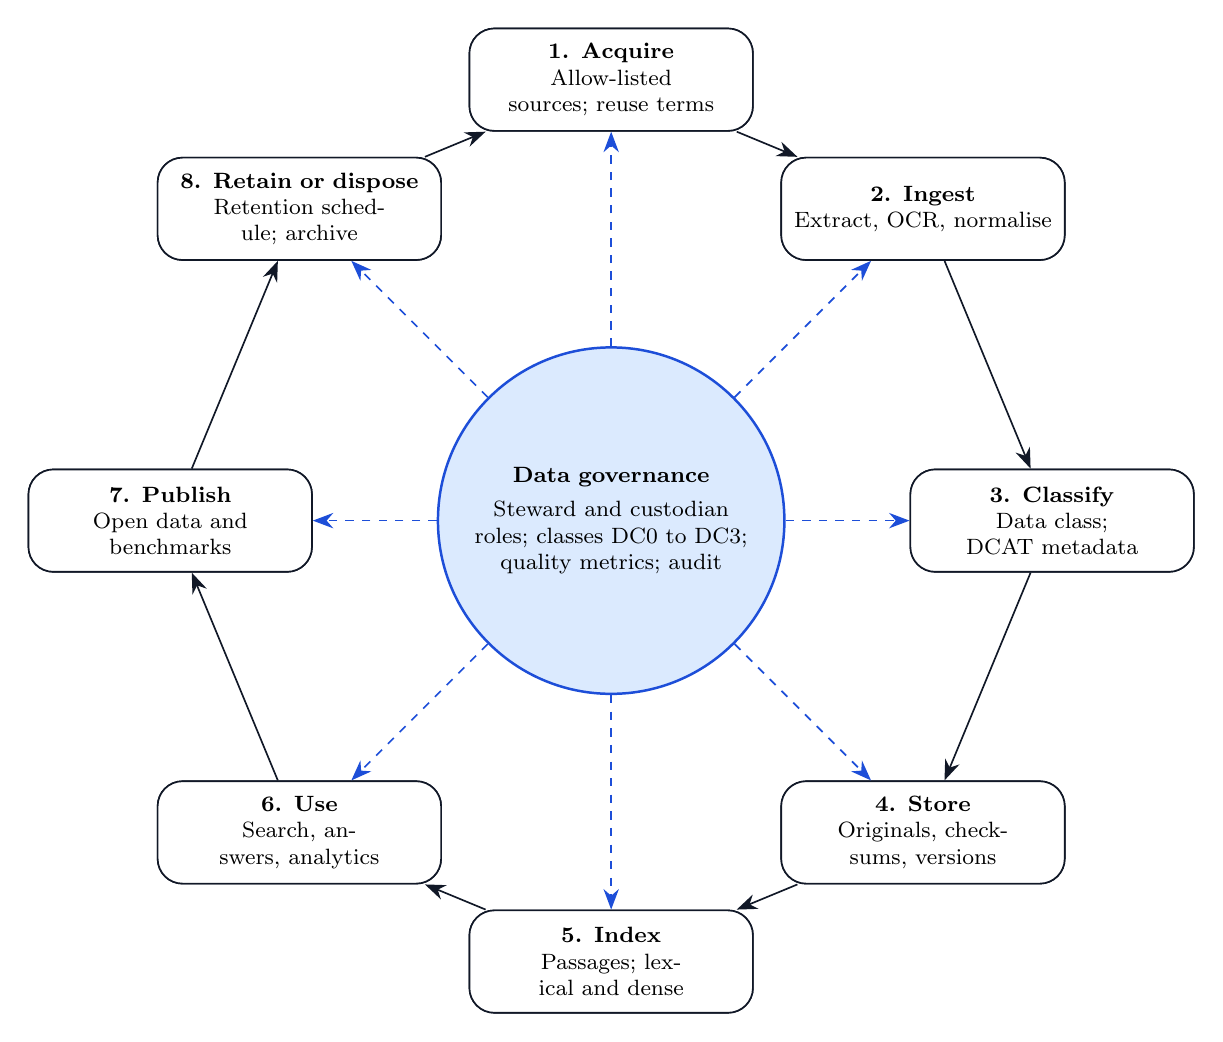
\begin{tikzpicture}
\node[key, circle, minimum size=44mm, text width=38mm, font=\footnotesize] (c) at (0,0) {\textbf{Data governance}\\[1mm]Steward and custodian roles; classes DC0 to DC3; quality metrics; audit};
\tikzset{st/.style={box, minimum width=36mm, minimum height=13mm, text width=33mm, font=\footnotesize}}
\foreach \i/\a in {1/90,2/45,3/0,4/-45,5/-90,6/-135,7/180,8/135} {
  \node[st] (s\i) at (\a:56mm) {};
}
\node[st] at (s1) {\textbf{1. Acquire}\\Allow-listed sources; reuse terms}; \node[st] at (s2) {\textbf{2. Ingest}\\Extract, OCR, normalise};
\node[st] at (s3) {\textbf{3. Classify}\\Data class; DCAT metadata}; \node[st] at (s4) {\textbf{4. Store}\\Originals, checksums, versions};
\node[st] at (s5) {\textbf{5. Index}\\Passages; lexical and dense}; \node[st] at (s6) {\textbf{6. Use}\\Search, answers, analytics};
\node[st] at (s7) {\textbf{7. Publish}\\Open data and benchmarks}; \node[st] at (s8) {\textbf{8. Retain or dispose}\\Retention schedule; archive};
\foreach \i/\j in {1/2,2/3,3/4,4/5,5/6,6/7,7/8,8/1} \draw[arr] (s\i) -- (s\j);
\foreach \i in {1,...,8} \draw[darr, draw=accent] (c) -- (s\i);
\end{tikzpicture}
\end{document}
